%====================================================================
% PREAMBLE
%====================================================================
\documentclass[11pt, spanish, open=any]{scrbook}

% --- Core Packages ---
\usepackage[T1]{fontenc}           % Use modern font encodings
\usepackage{lmodern}               % Use the Latin Modern font
\usepackage[utf8]{inputenc}        % For UTF-8 input
\usepackage[english]{babel}        % Language-specific typesetting
\usepackage{microtype}             % Improves justification and typography
\usepackage{csquotes}

% --- Arsclassica Styling ---
\usepackage{arsclassica}

% --- Mathematics Packages ---
\usepackage{amsmath}
\usepackage{mathtools}
\usepackage{amssymb}
\usepackage{amsfonts}
\usepackage{bm}                    % For bold math symbols, e.g., \bm{v}
\usepackage{derivative}            % For derivatives notation

% --- Graphics and Referencing ---
\usepackage{graphicx}              % For including images
\usepackage[capitalize]{cleveref}  % For smart cross-referencing (use \cref{})

% --- Bibliography ---
\usepackage[
    backend=biber,
    style=numeric-comp,
    sorting=none
]{biblatex}
\addbibresource{references.bib}    % Link the bibliography file

% --- Theorem-like Environments ---
\newtheorem{theorem}{Theorem}[chapter]
\newtheorem{definition}[theorem]{Definition} % Uses the same counter as theorem
\newtheorem{lemma}[theorem]{Lemma}
\newtheorem{proposition}[theorem]{Proposition}


%====================================================================
% DOCUMENT METADATA
%====================================================================
\title{Bitacoras del Seminario de Física Teórica}
\author{}
\date{2025}
\publishers{
    Programa Académico de Física \\
    Facultad de Ciencias Matemáticas y Naturales \\
    Universidad Distrital Francisco José de Caldas
}

%====================================================================
% DOCUMENT BODY
%====================================================================
\begin{document}

% --- Front Matter ---
\frontmatter
\maketitle
\tableofcontents

% --- Main Matter ---
\mainmatter

% --- NUEVA SECCIÓN DE PARTICIPANTES ---
\chapter{Participantes del Seminario}
En este seminario participaron:

\begin{itemize}
	\item Profesor Alfonso Leyva
	\item Yerly Zaudi Gomez Contreras
	\item Camilo Andres Huertas Archila
	\item Julian Leonardo Avila Martinez 
	\item Manuel Adriano Parada Ospina
	\item David Santiago Rodriguez Ortiz
	\item Eric Arciniegas Barreto
	\item Jose Luis Zamora Alvarado
	\item Laura Yeraldin Herrera Martinez
	\item Sebastian Rodriguez
	\item Juan Sebastian Acuña Tellez
\end{itemize}

 


\chapter{Problema de 2 cuerpos:}

\section{Goldstein, Capitulo 3:}
Considere un sistema de dos partículas $m_1$ y $m_2$ de la misma clase, con fuerzas centrales mutuas, cuyas posiciones están dadas en términos de los vectores $\vec{r}_1$ y $\vec{r}_2$. En primera, las fuerzas que actúan sobre cada partícula será función del vector distancia entre ellas definido por $\vec{r}=\vec{r}_2-\vec{r}_1$, por ende asociamos un potencial en función de la magnitud $r$ de forma $U(r,\dot{r},...)$, así nuestro sistema de 6 grados de libertad estará dado por el lagrangiano:
	
	\[
	L=T-U=\frac{1}{2}m_1\dot{r}_1^2+\frac{1}{2}m_2\dot{r}_2^2 - U(r,\dot{r},...)
	\]

	Ahora conviene escribir $\vec{r}_1$ y $\vec{r}_2$ en términos del centro de masa $\vec{R}$ y el vector $\vec{r}$, efectuando una transformación en las ecuaciones de Lagrange que preserva su forma, reescribimos entonces los vectores de la siguiente forma:
	
	\[
	\begin{array}{c}
		\vec{r}_1=\vec{R}+\vec{r'}_1\\\vec{r}_2=\vec{R}+\vec{r'}_2
	\end{array}
	\quad\quad\text{con}\quad\quad \vec{R}=\frac{m_1\vec{r}_1+m_2\vec{r}_2}{m_1+m_2}\quad \vec{r'}_1=-\frac{m_2}{m_1+m_2}\vec{r}\quad\vec{r'}_2=\frac{m_1}{m_1+m_2}\vec{r}
	\]
	
	Es necesario transformar el lagrangiano en función de $\vec{R}$ y $\vec{r}$ usando las ecuaciones de transformación previamente escritas. Notemos que, en el sistema primado donde se definen $\vec{r'}_1$ y $\vec{r'}_2$ (vectores que van del centro de masas hasta la partícula), el centro de masas coincide con el vector nulo:
	
	\[
	L=\frac{1}{2}m_1(\dot{R}^2+\dot{r'}^{2}_1)+\frac{1}{2}m_2(\dot{R}^2+\dot{r'}^{2}_2)+\dot{\vec{R}}\cdot\frac{d}{dt}(m_1\vec{r'}_1+m_2\vec{r'}_2) - U(r,\dot{r},...)
	\]
	
	Así el tercer termino es nulo y el lagrangiano toma la forma, en la que es necesario aplicar álgebra para dejarlo totalmente en función de $\vec{r}$:
	
	\[
	L=\frac{1}{2}(m_1+m_2)\dot{R}^{2}+\frac{1}{2}(m_1\dot{r'}^{2}_1+m_2\dot{r'}^{2}_2)-U(r,\dot{r},...)
	\]
	
	\[
	\dot{r'}^{2}_1=\frac{m_2^{2}}{(m_1+m_2)^{2}}\dot{r}^{2}\quad\dot{r'}^{2}_2=\frac{m_1^{2}}{(m_1+m_2)^{2}}\dot{r}^{2}\quad\quad m_1\dot{r'}^{2}_1+m_2\dot{r'}^{2}_2=\frac{m_1m_2}{m_1+m_2}\left[\frac{m_2\dot{r}^2+m_1\dot{r}^2}{m_1+m_2}\right]
	\]
	
	\[
	L=\frac{1}{2}(m_1+m_2)\dot{R}^{2}+\frac{1}{2}\frac{m_1m_2}{m_1+m_2}\dot{r}^2-U(r,\dot{r},...)
	\]
	
	Podemos notar que $R$ es cíclica, es decir, la lagrangiana no contiene $R$ (no tomar como definición) y por ende tendrá una cantidad de movimiento que se conserva, lo restante define un sistema de una sola partícula (con 3 grados de libertad) de masa reducida $\mu$ cuya posición esta definida por $\vec{r}$:
	
	\[
	L=\frac{1}{2}\frac{m_1m_2}{m_1+m_2}\dot{r}^2-U(r,\dot{r},...)=\frac{1}{2}\mu\dot{r}^2-U(r,\dot{r},...)
	\]
	
	Consideraremos ahora fuerzas conservativas, es decir $U=U(r)$, y la simetría esférica del sistema, note que se pueden hacer rotaciones alrededor de la esfera que define el vector $r$ sin alterar el lagrangiano del sistema, es decir, se conserva el momentum angular total:
	
	\[
	\vec{L}=\vec{r}\times\vec{p}\quad\quad \vec{L}(l,\theta,\phi)
	\]
	
	De aquí se sigue que $\vec{r}$ esta dado sobre el plano que define $\vec{L}$, si se fija $\theta$ y $\phi$ de $\vec{L}$ el numero de grados de libertad disminuye a 2 y contamos así con dos cantidades conservadas para solucionar el problema, $E$ y $l$. Ahora escribimos el lagrangiano en coordenadas polares y junto a las dos ecuaciones de movimiento:
	
	\[
	L=T-U=\frac{1}{2}\mu(\dot{r}^2+r^2\dot{\theta}^2)-U(r)
	\]
	
	Notamos que $\theta$ es cíclica pero no se puede ignorar, aunque igual tiene una cantidad conservada asociada $p_\theta\equiv l$, esta primera ecuación de movimiento se puede escribir de manera tal que se llegue a una de las leyes de Kepler, áreas iguales en tiempos iguales:
	
	\[
	\dot{p_\theta}=\frac{d}{dt}\left(\mu r^2\dot{\theta}\right)=0\quad\quad\frac{d}{dt}\left(\frac{1}{2}rr\dot{\theta}\right)=0\quad\quad dA=\frac{1}{2}rrd\theta\quad\Longrightarrow\frac{d}{dt}\left(\frac{dA}{dt}\right)=0
	\]
	
	En cuanto a la segunda ecuación de movimiento, es posible reescribirla usando el momentum angular $l=mr^2\dot{\theta}$, donde $f(r)$ es la fuerza efectuada sobre la partícula que no esta en el centro de coordenadas:
	
	\[
	\mu\ddot{r}-\mu r\dot{\theta}^2=-\frac{\partial U}{\partial r}=f(r)\quad\quad\mu\ddot{r}-\frac{l^2}{\mu r^3}=f(r)\quad\Longrightarrow\quad\mu\ddot{r}=f(r)+\frac{l^2}{\mu r^3}
	\]  
	El segundo termino lo podemos reescribir como la derivada respecto a $r$ de cierta cantidad, en cuanto al primer termino, si multiplicamos la ecuación por $\dot{r}$, es posible escribirlo como una derivada respecto al tiempo:
	
	\[
	f(r)+\frac{l^2}{\mu r^3}=-\frac{d}{dr}\left(U+\frac{1}{2}\frac{l^2}{\mu r^2}\right)\quad\quad\mu\ddot{r}\dot{r}=\frac{d}{dt}\left(\frac{1}{2}\mu\dot{r}^2\right)
	\]
	\[
	\mu\ddot{r}\dot{r}=\left(f(r)+\frac{l^2}{\mu r^3}\right)\dot{r}\quad\Longrightarrow\quad\frac{d}{dt}\left(\frac{1}{2}\mu\dot{r}^2\right)=-\frac{d}{dr}\left(U+\frac{1}{2}\frac{l^2}{\mu r^2}\right)\frac{dr}{dt}
	\]
	
	\[
	\frac{d}{dt}\left(\frac{1}{2}\mu\dot{r}^2+U+\frac{1}{2}\frac{l^2}{\mu r^2}\right)=0
	\]
	
	Es así como llegamos a otra cantidad conservada que ya mencionamos en algún momento, la energía $E$. Es importante notar que ya hicimos la primera integral de cada una de las ecuaciones de movimiento, y no fue necesario acudir a los valore iniciales $\dot{r}_0$ y $\dot{\theta}_0$, es posible efectuar la segunda integral para las dos ecuaciones y determinar el estado del sistema con las cantidades $(E,l,r_0,\theta_0)$.


\section{Simmons, Seccion 21:}
\subsection{La ley de la gravitación de Newton y el movimiento de los planetas}
\textbf{Propósito:} Deducir las leyes de Kepler a partir de la ley de la gravitación universal de Newton. Para ello, se analiza el movimiento de una partícula de masa $m$ (un planeta) bajo la atracción de una partícula fija de masa $M$ mucho mayor (el sol).

\begin{figure}[htbp]
    \centering
    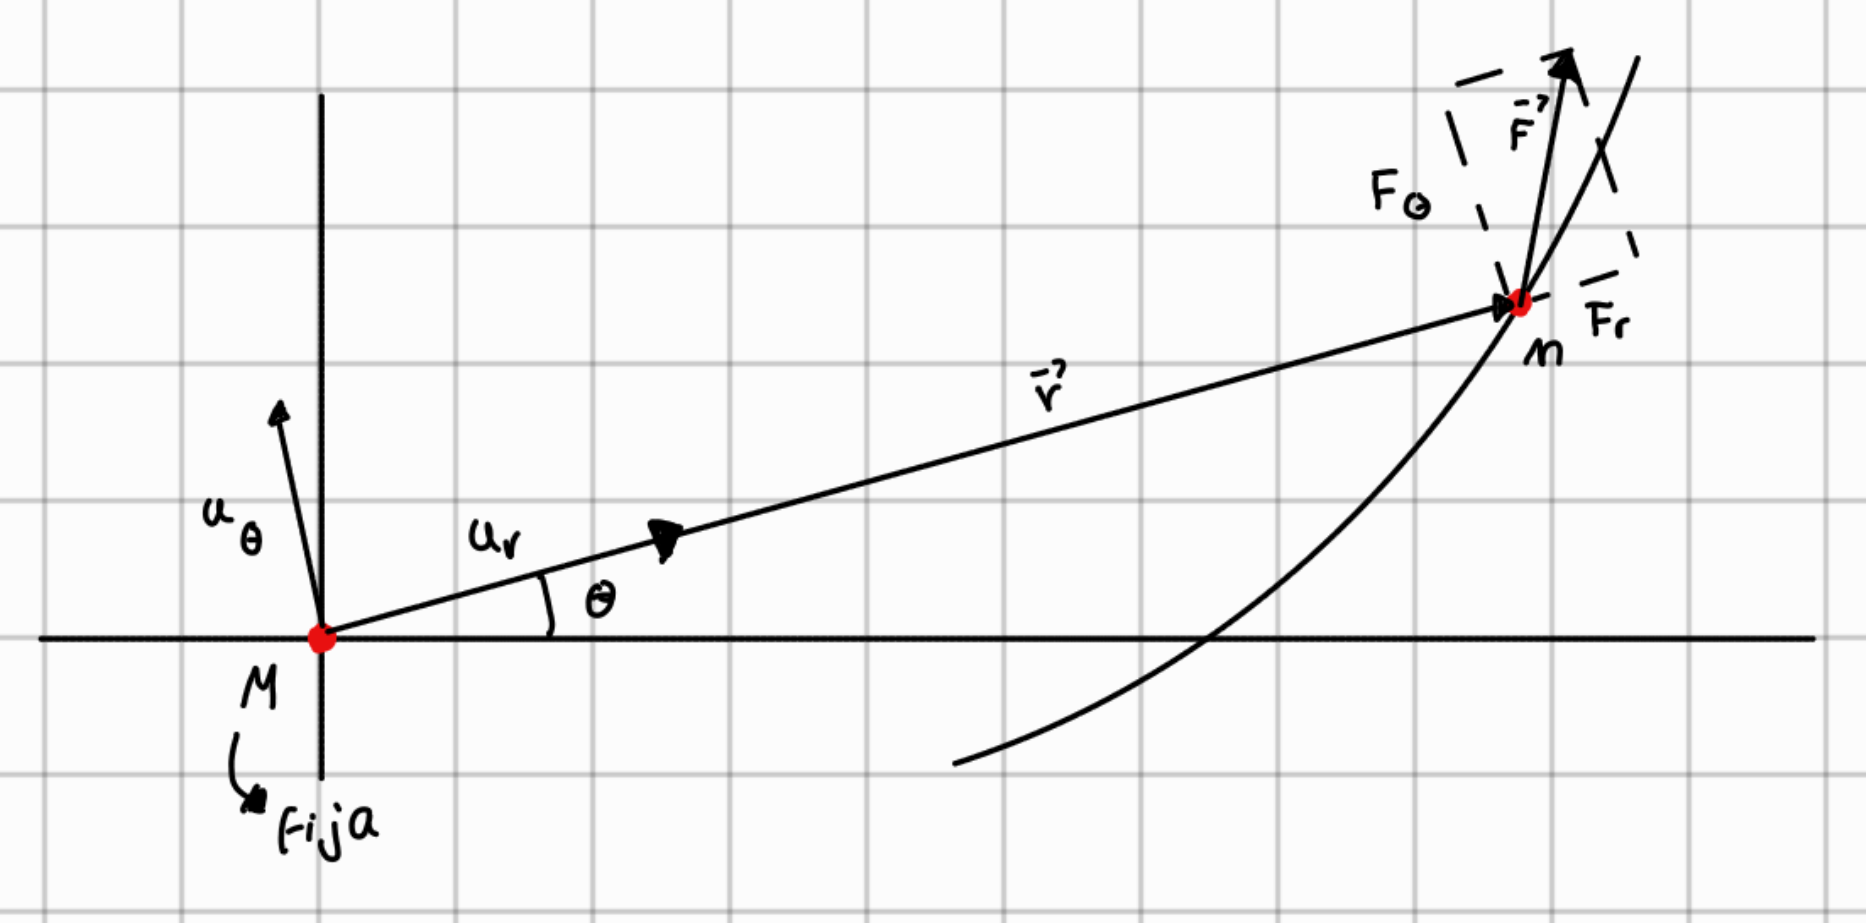
\includegraphics[width=0.8\textwidth]{./Sessions/Two-Body-Problem/Images/simmons-img1.png}
    \caption{Diagrama de cuerpo libre para el problema de dos cuerpos.}
    \label{fig:dcl_2cuerpos}
\end{figure}

En problemas de movimiento bajo una fuerza dirigida a un punto fijo, conviene descomponer los vectores en componentes radiales y perpendiculares a esta. El vector posición es:
\[ \vec{r} = r\vec{u}_r \]
cuyo vector unitario es:
\[ \vec{u}_r = \cos\theta \hat{i} + \sin\theta \hat{j} \]
y su vector perpendicular, en la dirección de $\theta$ creciente, es:
\[ \frac{d\vec{u}_r}{d\theta} = -\sin\theta \hat{i} + \cos\theta \hat{j} = \vec{u}_\theta \]
De la derivación se obtienen las relaciones esenciales:
\[ \frac{d\vec{u}_r}{d\theta} = \vec{u}_\theta \quad \text{y} \quad \frac{d\vec{u}_\theta}{d\theta} = -\vec{u}_r \]
Estas relaciones nos permiten obtener los vectores velocidad y aceleración.
\[ \vec{v} = \frac{d\vec{r}}{dt} = \frac{d}{dt}(r\vec{u}_r) = \frac{dr}{dt}\vec{u}_r + r\frac{d\vec{u}_r}{dt} \]
Por regla de la cadena, ya que $\vec{u}_r$ depende de $\theta$ y $\theta$ de $t$:
\[ \vec{v} = \frac{dr}{dt}\vec{u}_r + r\frac{d\vec{u}_r}{d\theta}\frac{d\theta}{dt} \]
\[ \vec{v} = \frac{dr}{dt}\vec{u}_r + r\frac{d\theta}{dt}\vec{u}_\theta \]
Y el vector aceleración, tras un cálculo directo a partir de $\vec{v}$, es:
\[ \vec{a} = \left[\frac{d^2r}{dt^2} - r\left(\frac{d\theta}{dt}\right)^2\right]\vec{u}_r + \left[r\frac{d^2\theta}{dt^2} + 2\frac{dr}{dt}\frac{d\theta}{dt}\right]\vec{u}_\theta \]
Si $\vec{F}$ es la fuerza que actúa sobre $m$, entonces $\vec{F} = F_r\vec{u}_r + F_\theta\vec{u}_\theta$.
Recordando la segunda ley de Newton, $\vec{F}=m\vec{a}$, se concluye que:
\begin{align}
    m\left(r\frac{d^2\theta}{dt^2} + 2\frac{dr}{dt}\frac{d\theta}{dt}\right) &= F_\theta \tag{1} \\
    m\left(\frac{d^2r}{dt^2} - r\left(\frac{d\theta}{dt}\right)^2\right) &= F_r \tag{2}
\end{align}
Estas ecuaciones diferenciales gobiernan el movimiento de la partícula, sea cual sea la naturaleza de la fuerza.

\subsection{Fuerzas centrales y segunda ley de Kepler}
Se dice que $\vec{F}$ es una fuerza central si está siempre dirigida a lo largo de la línea que une la partícula con el origen, es decir, si no tiene componente perpendicular, $F_\theta=0$. Bajo esta hipótesis, la ecuación (1) queda como:
\[ r\frac{d^2\theta}{dt^2} + 2\frac{dr}{dt}\frac{d\theta}{dt} = 0 \]
Multiplicando por $r$, la expresión se puede reconocer como la derivada de un producto:
\[ \frac{d}{dt}\left(r^2\frac{d\theta}{dt}\right) = 0 \]
Integrando ambos lados, se obtiene que:
\begin{equation} r^2 \frac{d\theta}{dt} = h \tag{3} \end{equation}
donde $h$ es una constante de integración. Si $A=A(t)$ es el área barrida por el radio vector, el diferencial de área es $dA = \frac{1}{2}r^2d\theta$. La tasa con que se barre el área es:
\[ \frac{dA}{dt} = \frac{1}{2}r^2\frac{d\theta}{dt} = \frac{h}{2} \]
Como $h$ es constante, la velocidad areolar también lo es. Al integrar entre dos instantes de tiempo, se obtiene que $A(t_2) - A(t_1) = \frac{h}{2}(t_2-t_1)$. Esta es la \textbf{Segunda Ley de Kepler}: el radio vector barre áreas iguales en intervalos iguales de tiempo\footnote{Kepler (1571-1630) destiló sus tres leyes tras trabajar incesantemente durante veinte años con la gran cantidad de datos observacionales heredados del astrónomo danés Tycho Brahe.}.

\subsection{Fuerzas gravitacionales centrales y primera ley de Kepler}
Ahora se especializa el análisis para una fuerza central atractiva cuya magnitud sigue la ley de la gravitación de Newton:
\[ F_r = -G\frac{Mm}{r^2} = -\frac{km}{r^2} \]
donde $k=GM$. La ecuación (2) pasa a ser:
\begin{equation} \frac{d^2r}{dt^2} - r\left(\frac{d\theta}{dt}\right)^2 = -\frac{k}{r^2} \tag{4} \end{equation}
El siguiente paso es obtener la ecuación de la órbita en forma polar $r=f(\theta)$, para lo cual se debe eliminar el tiempo $t$ y considerar $\theta$ como la variable independiente. Usando la ecuación (3) en la (4):
\begin{equation} \frac{d^2r}{dt^2} - \frac{h^2}{r^3} = -\frac{k}{r^2} \tag{5} \end{equation}
El libro de Simmons describe este paso como "difícil de motivar, ya que requiere considerable ingenio técnico". La presencia de potencias de $1/r$ sugiere el cambio de variable $z=1/r$. Se expresa $\frac{d^2r}{dt^2}$ en términos de $z$ y $\theta$:
\[ \frac{dr}{dt} = \frac{d}{dt}\left(\frac{1}{z}\right) = -h\frac{dz}{d\theta} \]
\[ \frac{d^2r}{dt^2} = -h^2z^2\frac{d^2z}{d\theta^2} \]
Al insertar esta expresión en (5) y sustituir $r=1/z$, queda:
\[ -h^2z^2\frac{d^2z}{d\theta^2} - h^2z^3 = -kz^2 \]
que se simplifica a la EDO lineal:
\[ \frac{d^2z}{d\theta^2} + z = \frac{k}{h^2} \]
La solución general es inmediata:
\begin{equation} z = A\sin\theta + B\cos\theta + \frac{k}{h^2} \tag{6} \end{equation}
Por simplificar, se desplaza el eje polar de modo que $r$ sea mínimo (perihelio) cuando $\theta=0$. Esto implica que $z$ es máximo, y por tanto $\frac{dz}{d\theta}|_{\theta=0}=0$, lo cual fuerza a que $A=0$. Despejando $r=1/z$:
\[ r = \frac{h^2/k}{1 + (Bh^2/k)\cos\theta} \]
Si se define la excentricidad $e = Bh^2/k$ (una constante positiva), la ecuación de la órbita se convierte en:
\begin{equation} r = \frac{h^2/k}{1+e\cos\theta} \tag{7} \end{equation}
Esta es la ecuación polar de una sección cónica con foco en el origen y excentricidad $e$. Puesto que los planetas permanecen en el sistema solar, sus órbitas son cerradas y la elipse ($e<1$) es la única posibilidad. Esto constituye la \textbf{Primera Ley de Kepler}: la órbita de cualquier planeta es una elipse con uno de sus focos en el Sol.

\subsection{Significado físico de la excentricidad y Tercera Ley de Kepler}
La energía total del sistema $E$ (cinética + potencial) es constante:
\[ E = \frac{1}{2}mv^2 - \frac{km}{r} \]
Se puede demostrar que la excentricidad depende directamente de la energía total del sistema:
\[ e = \sqrt{1 + E\left(\frac{2h^2}{mk^2}\right)} \]
Resulta claro que la naturaleza de la órbita queda completamente caracterizada por su energía total $E$. La órbita es una elipse si $E<0$, una parábola si $E=0$ y una hipérbola si $E>0$. Los planetas del sistema solar tienen energía negativa.

Para la Tercera Ley, se relaciona la dinámica con la geometría de la elipse. En astronomía, el semieje mayor $a$ se conoce como la distancia media. Es la semisuma de las distancias máxima y mínima de $r$. Un cálculo muestra que:
\[ a = \frac{h^2}{k(1-e^2)} \]
Usando la propiedad geométrica de la elipse $b^2 = a^2(1-e^2)$, se encuentra una relación para el semieje menor $b$:
\[ b^2 = \frac{h^2 a}{k} \]
Si $T$ es el período de la órbita, y el área de la elipse es $\pi ab$, de la segunda ley de Kepler se sigue que $\pi ab = hT/2$. Elevando al cuadrado y sustituyendo $b^2$:
\[ T^2 = \frac{4\pi^2 a^2 b^2}{h^2} = \frac{4\pi^2 a^2}{h^2}\left(\frac{h^2a}{k}\right) = \left(\frac{4\pi^2}{k}\right)a^3 \]
Como $k=GM$ es la misma constante para todos los planetas, se obtiene la \textbf{Tercera Ley de Kepler}: los cuadrados de los períodos de revolución de los planetas son proporcionales a los cubos de sus distancias medias.



% --- Back Matter ---
% Contains appendices, bibliography, index.
\backmatter

\printbibliography % This command prints the bibliography

\end{document}
